%=====================================================================
%  We Know Group | Kato Kiosk Installation Guide
%  Create, Configure & Install  --  Version 1.0
%
%  Branding per "We Know Group Brand Guidelines V2 2023":
%    - Primary colours: Graphite #121212, Azure #00A6D3, White
%    - Secondary: Sky Blue #E5F1F9, Sea Blue #008BB2, Night Blue #0C2752
%    - Greys: Night #575A5C, Mid #ADADAD, Light #F4F4F4
%    - Typeface: Circular Pro (approximated here with Inter, the licensed
%      brand stand-in used in the WeKnow Employee Handbook)
%    - Logos are the official WeKnow assets in images/ -- never redrawn.
%
%  Style mirrors the certified "FreedomPay Windows FCC -- Auth & Capture"
%  integration guide (CER-3425) so the two documents read as a set.
%=====================================================================
\documentclass[a4paper,10pt]{article}

%---------------------------------------------------------------------
% Fonts & encoding -- Inter (brand stand-in for Circular Pro)
%---------------------------------------------------------------------
\usepackage[T1]{fontenc}
\usepackage[utf8]{inputenc}
\usepackage[sfdefault]{inter}
\renewcommand{\familydefault}{\sfdefault}
\usepackage{microtype}

%---------------------------------------------------------------------
% Layout
%---------------------------------------------------------------------
\usepackage[a4paper,margin=20mm,top=28mm,bottom=22mm,headheight=20pt,headsep=14pt]{geometry}
\usepackage{graphicx}
\graphicspath{{images/}}
\usepackage[table]{xcolor}
\usepackage{tikz}
\usetikzlibrary{arrows.meta,positioning,calc,shapes.misc,fit,backgrounds}
\usepackage{tcolorbox}
\tcbuselibrary{skins,breakable}
\usepackage{booktabs}
\usepackage{array}
\usepackage{tabularx}
\usepackage{enumitem}
\usepackage{fancyhdr}
\usepackage{titlesec}
\usepackage{listings}
\usepackage{float}
\usepackage{lastpage}
\usepackage{amssymb}
\usepackage{caption}
\usepackage[hidelinks,colorlinks=true,urlcolor=weknowsea,linkcolor=weknownight]{hyperref}

%---------------------------------------------------------------------
% We Know Group palette (Brand Guidelines V2 2023, Section 3)
%---------------------------------------------------------------------
\definecolor{weknowazure}{HTML}{00A6D3}     % Hero colour
\definecolor{weknowgraphite}{HTML}{121212}
\definecolor{weknowsky}{HTML}{E5F1F9}
\definecolor{weknowsea}{HTML}{008BB2}
\definecolor{weknownight}{HTML}{0C2752}
\definecolor{weknowgreyN}{HTML}{575A5C}
\definecolor{weknowgreyM}{HTML}{ADADAD}
\definecolor{weknowgreyL}{HTML}{F4F4F4}
\definecolor{weknowazure80}{HTML}{33B8DC}    % Azure tints (brand: tint Azure only)
\definecolor{weknowazure60}{HTML}{66CAE5}
\definecolor{weknowazure40}{HTML}{99DBED}
\definecolor{weknowazure20}{HTML}{CCEDF6}

%---------------------------------------------------------------------
% Headers / footers
%---------------------------------------------------------------------
\pagestyle{fancy}
\fancyhf{}
\fancyhead[L]{\footnotesize\color{weknowgreyN}\nouppercase{\leftmark}}
\fancyhead[R]{\raisebox{-0.35\height}{
\includegraphics[height=15pt]{wkg-logo-horizontal}}}
\renewcommand{\headrulewidth}{0.8pt}
\renewcommand{\headrule}{\hbox to\headwidth{\color{weknowazure}\leaders\hrule height \headrulewidth\hfill}}
\fancyfoot[L]{\scriptsize\color{weknowgreyN}Internal --- We Know Group}
\fancyfoot[C]{\scriptsize\color{weknowgreyN}Kato Kiosk Installation Guide}
\fancyfoot[R]{\scriptsize\color{weknowgreyN}Page \thepage\ of \pageref{LastPage}}
\renewcommand{\footrulewidth}{0.4pt}
\renewcommand{\footrule}{\hbox to\headwidth{\color{weknowgreyM}\leaders\hrule height \footrulewidth\hfill}}

%---------------------------------------------------------------------
% Section styling
%---------------------------------------------------------------------
\titleformat{\section}
  {\color{weknowgraphite}\LARGE\bfseries}
  {\color{weknowazure}\thesection}{0.7em}{}
  [{\vspace{3pt}\color{weknowazure}\titlerule[1.4pt]}]
\titleformat{\subsection}
  {\color{weknowsea}\Large\bfseries}
  {\color{weknowazure}\thesubsection}{0.6em}{}
\titlespacing*{\section}{0pt}{20pt}{12pt}
\titlespacing*{\subsection}{0pt}{16pt}{6pt}
\renewcommand{\sectionmark}[1]{\markright{\thesection\quad #1}}

%---------------------------------------------------------------------
% Captions
%---------------------------------------------------------------------
\captionsetup{font=small,labelfont={bf,color=weknownight},
              textfont={color=weknowgreyN},skip=5pt}

%---------------------------------------------------------------------
% Screenshot helper -- \screenshot[width fraction]{file}{caption}
%---------------------------------------------------------------------
\newcommand{\screenshot}[3][0.72]{%
  \begin{figure}[H]
    \centering
    \setlength{\fboxsep}{0pt}\setlength{\fboxrule}{0.6pt}%
    {\color{weknowgreyM}\fbox{\includegraphics[width=#1\linewidth]{#2}}}%
    \caption{#3}
  \end{figure}}

%---------------------------------------------------------------------
% Callout boxes
%---------------------------------------------------------------------
\newtcolorbox{wkinfo}[1][]{%
  enhanced,breakable,colback=weknowsky,colframe=weknowazure,
  boxrule=0pt,leftrule=2.5pt,arc=1.5pt,
  fonttitle=\bfseries,coltitle=weknownight,title={#1},
  left=6pt,right=6pt,top=5pt,bottom=5pt}
\newtcolorbox{wkwarn}[1][]{%
  enhanced,breakable,colback=weknowgreyL,colframe=weknownight,
  boxrule=0pt,leftrule=2.5pt,arc=1.5pt,
  fonttitle=\bfseries,coltitle=weknownight,title={#1},
  left=6pt,right=6pt,top=5pt,bottom=5pt}

%---------------------------------------------------------------------
% Code listings
%---------------------------------------------------------------------
\lstdefinestyle{wkcode}{
  basicstyle=\ttfamily\footnotesize\color{weknowgraphite},
  backgroundcolor=\color{weknowgreyL},
  frame=single, framerule=0pt, rulecolor=\color{weknowgreyL},
  breaklines=true, breakatwhitespace=false,
  columns=fullflexible, keepspaces=true,
  aboveskip=8pt, belowskip=8pt, xleftmargin=6pt, framexleftmargin=6pt}
\lstset{style=wkcode}

\newcolumntype{L}[1]{>{\raggedright\arraybackslash}p{#1}}
\setlist{nosep,itemsep=4pt}

% Shorthands
\newcommand{\wpath}[1]{{\ttfamily\small #1}}
\newcommand{\tick}{{\color{weknowsea}$\checkmark$}}
\newcommand{\emptybox}{{\color{weknowgreyM}$\square$}}

\begin{document}

%=====================================================================
% COVER
%=====================================================================
\begin{titlepage}
\thispagestyle{empty}
\begin{tikzpicture}[remember picture,overlay]
  % --- 'Wink' echo: symmetric Azure-tint rounded squares framing the top ---
  \fill[weknowazure20,rounded corners=8mm]
       ([xshift=-46mm,yshift=-46mm]current page.north east) rectangle
       ([xshift=14mm,yshift=-8mm]current page.north east);
  \fill[weknowazure40,rounded corners=5mm]
       ([xshift=-30mm,yshift=-40mm]current page.north east) rectangle
       ([xshift=8mm,yshift=-13mm]current page.north east);
  \fill[weknowazure20,rounded corners=8mm]
       ([xshift=-14mm,yshift=-46mm]current page.north west) rectangle
       ([xshift=46mm,yshift=-8mm]current page.north west);
  \fill[weknowazure40,rounded corners=5mm]
       ([xshift=-8mm,yshift=-40mm]current page.north west) rectangle
       ([xshift=30mm,yshift=-13mm]current page.north west);

  % --- Large centred WeKnow logo (stacked variant) = the hero ---
  \node[anchor=north] at ([yshift=-50mm]current page.north)
       {
\includegraphics[width=52mm]{wkg-logo-stacked}};

  % --- Centred title / Azure hero rule / subtitle ---
  \node[anchor=north,align=center,text width=185mm]
       at ([yshift=-126mm]current page.north)
       {{\color{weknowgraphite}\fontsize{26}{31}\selectfont\bfseries Kato Kiosk Installation Guide}\\[11pt]
        {\color{weknowazure}\rule{42mm}{2pt}}\\[11pt]
        {\color{weknowsea}\fontsize{16}{20}\selectfont Create, configure and install a kiosk --- step by step}};

  % --- Metadata panel ---
  \node[anchor=north, fill=weknowsky, rounded corners=3mm,
        inner xsep=12mm, inner ysep=8mm]
       at ([yshift=-174mm]current page.north)
       {\renewcommand{\arraystretch}{1.5}%
        \begin{tabular}{@{}l@{\hspace{12mm}}l@{}}
          {\color{weknowsea}\bfseries Version} & {\color{weknowgraphite}1.0}\\
          {\color{weknowsea}\bfseries Date} & {\color{weknowgraphite}August 2026}\\
          {\color{weknowsea}\bfseries Classification} & {\color{weknowgraphite}Internal}\\
          {\color{weknowsea}\bfseries Prepared by} & {\color{weknowgraphite}We Know Group --- Integrations}\\
          {\color{weknowsea}\bfseries Audience} & {\color{weknowgraphite}Field installers \& operations}\\
        \end{tabular}};

  % --- Confidentiality notice ---
  \node[anchor=south,align=center,text width=150mm]
       at ([yshift=20mm]current page.south)
       {{\color{weknowgreyM}\rule{55mm}{0.4pt}}\\[8pt]
        {\color{weknowgreyN}\footnotesize This document contains confidential and proprietary
         information belonging to We Know Group. It is intended solely for internal use and may
         not be reproduced or distributed without prior written consent.}};
\end{tikzpicture}
\end{titlepage}

%=====================================================================
% HOW TO USE THIS GUIDE
%=====================================================================
\section*{How to use this guide}
\markright{How to use this guide}

Follow the six stages \textbf{in order}. Each stage ends with a
\emph{Done when} line --- do not move on until it is true. If a step
fails, jump to \S\ref{sec:trouble} (\emph{When things go wrong}) rather
than improvising.

\begin{figure}[H]
\centering
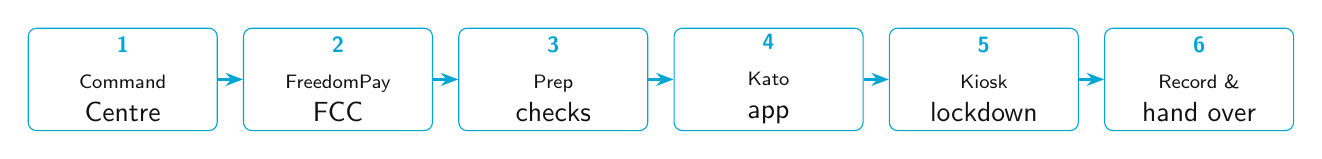
\begin{tikzpicture}[
  chip/.style={draw=weknowazure,fill=white,rounded corners=3pt,
               minimum width=24mm,minimum height=13mm,align=center,
               inner sep=2pt,text=weknowgraphite},
  arr/.style={-{Stealth[length=2.2mm]},thick,weknowazure},
  node distance=3.2mm]

  \node[chip] (s1) {\textcolor{weknowazure}{\footnotesize\bfseries 1}\\[1pt]\scriptsize Command\\Centre};
  \node[chip,right=of s1] (s2) {\textcolor{weknowazure}{\footnotesize\bfseries 2}\\[1pt]\scriptsize FreedomPay\\FCC};
  \node[chip,right=of s2] (s3) {\textcolor{weknowazure}{\footnotesize\bfseries 3}\\[1pt]\scriptsize Prep\\checks};
  \node[chip,right=of s3] (s4) {\textcolor{weknowazure}{\footnotesize\bfseries 4}\\[1pt]\scriptsize Kato\\app};
  \node[chip,right=of s4] (s5) {\textcolor{weknowazure}{\footnotesize\bfseries 5}\\[1pt]\scriptsize Kiosk\\lockdown};
  \node[chip,right=of s5] (s6) {\textcolor{weknowazure}{\footnotesize\bfseries 6}\\[1pt]\scriptsize Record \&\\hand over};

  \draw[arr] (s1) -- (s2);
  \draw[arr] (s2) -- (s3);
  \draw[arr] (s3) -- (s4);
  \draw[arr] (s4) -- (s5);
  \draw[arr] (s5) -- (s6);
\end{tikzpicture}
\caption{The six stages. Stages 1--2 can be done in either order, but stage 3 needs both complete.}
\end{figure}

\begin{wkinfo}[Golden rules]
\begin{itemize}
  \item The \textbf{API key is shown once}. Copy it the moment you
        generate it, or you will have to generate a new one.
  \item Never mix UAT and Production endpoints on the same machine.
  \item After changing any FreedomPay config file, \textbf{restart the
        services} --- nothing takes effect until you do.
  \item Do not skip the prep checks. They are what stops a half-built
        kiosk being marked live.
\end{itemize}
\end{wkinfo}

\tableofcontents
\clearpage

%=====================================================================
% 1  BEFORE YOU START
%=====================================================================
\section{Before you start}

\subsection{What you need in your hand}

\begin{center}
\renewcommand{\arraystretch}{1.35}\small
\begin{tabularx}{\textwidth}{L{44mm} X}
\rowcolor{weknownight}\color{white}\textbf{Item} &
\color{white}\textbf{Where it comes from}\\
Command Centre login &
\href{https://command.weknow.technology}{command.weknow.technology} --- ask
your manager if you do not have an account.\\
\rowcolor{weknowgreyL}
Kiosk hardware &
On site, unboxed, powered, with printer, PDQ (card terminal), sensors and
scanners connected.\\
Workstation serial &
The \wpath{WKG-POS-XXX} label on the machine. You will type this in twice
--- get it right.\\
\rowcolor{weknowgreyL}
FreedomPay Store ID \& Terminal ID &
FreedomPay boarding team, per property.\\
FCC installer + UK config/PAL bundle &
Internal mirror: \wpath{https://dev.weknowlondon.uk/SSM/freedompay/}\\
\rowcolor{weknowgreyL}
Kato installer &
\wpath{Kiosk Setup 1.0.0.exe} (or later) from the release share.\\
Windows accounts on the machine &
\wpath{WKGAdmin} (admin work) and \wpath{SelfBooker} (the account the
kiosk runs as).\\
\end{tabularx}
\end{center}

\subsection{Information the site must give you first}

If any of these are missing, the kiosk cannot be configured. Chase them
\emph{before} you travel.

\begin{center}
\renewcommand{\arraystretch}{1.25}\small
\begin{tabularx}{\textwidth}{X X}
\rowcolor{weknowgreyL}
\emptybox\ Request owner & \emptybox\ Default language (kiosk + PDQ)\\
\emptybox\ Hotel name & \emptybox\ Currency\\
\rowcolor{weknowgreyL}
\emptybox\ Hotel address & \emptybox\ Relevant airports\\
\emptybox\ RPS customer code & \emptybox\ Default Uber suggestions\\
\rowcolor{weknowgreyL}
\emptybox\ Outlet code & \emptybox\ Products for the home screen\\
\emptybox\ Which products to enable & \emptybox\ Timezone\\
\end{tabularx}
\end{center}

\begin{wkwarn}[Two identifiers, two different things]
The \textbf{Kiosk ID} is a UUID generated by Command Centre and is used by
the app to identify itself. The \textbf{Workstation ID} is the physical
machine label (\wpath{WKG-POS-XXX}). Both go into the install command in
stage 4 --- do not swap them.
\end{wkwarn}

%=====================================================================
% 2  STAGE 1
%=====================================================================
\clearpage
\section{Stage 1 --- Create the kiosk in Command Centre}\label{sec:cc}

Do this from any machine with a browser. You are creating the kiosk
\emph{record} and collecting the two credentials the app will need.

\begin{enumerate}
  \item Open \href{https://command.weknow.technology}{Command Centre}
        and sign in.

  \item Go to \href{https://command.weknow.technology/locations}{Locations}
        and create the location, working down the hierarchy:
        \textbf{Country $\rightarrow$ Region $\rightarrow$ City $\rightarrow$
        Location}. Open the new location and \textbf{copy the Location ID}
        --- you need it in stage 6.
\end{enumerate}

\screenshot[0.60]{cc-location-id}{The location Overview tab. Use the copy icon next to \textbf{Location ID}.}

\begin{enumerate}\setcounter{enumi}{2}
  \item \emph{Only if required:} create a group from
        \href{https://command.weknow.technology/groups}{Groups}. Groups
        are either \textbf{location groups} or \textbf{kiosk groups} ---
        use them to apply shared config to several sites or several
        kiosks at once. Skip this for a single standalone kiosk.

  \item Go to \textbf{Kiosks} and select \textbf{Add Kiosk}. Fill in:
    \begin{itemize}
      \item \textbf{Name} --- how the kiosk will be referred to
            operationally, e.g.\ \emph{T2/T3 Tunnel - 2}.
      \item \textbf{Serial number} --- the workstation label,
            e.g.\ \wpath{WKG-POS-617}.
      \item \textbf{Hardware model} --- e.g.\ \emph{K10/20}.
      \item \textbf{Firmware version} --- e.g.\ \emph{1.0.0}.
    \end{itemize}
    Then select \textbf{Create Kiosk}.
\end{enumerate}

\screenshot[0.52]{cc-add-kiosk}{Add Kiosk. The kiosk is created unassigned --- it is tied to a location later, by the installation record.}

\begin{enumerate}\setcounter{enumi}{4}
  \item The new kiosk appears with status \textbf{In Stock}. That is
        expected --- it stays In Stock until it is installed.

  \item Open the kiosk, stay on the \textbf{Overview} tab and
        \textbf{copy the Kiosk ID}.
\end{enumerate}

\screenshot[0.58]{cc-kiosk-id}{Kiosk Overview --- copy the \textbf{Kiosk ID}. This is the \wpath{/KIOSKID} value in stage 4.}

\begin{enumerate}\setcounter{enumi}{6}
  \item Switch to the \textbf{API keys} tab and select
        \textbf{Generate API key}. This is the key the kiosk uses to
        authenticate to the server.
\end{enumerate}

\screenshot[0.56]{cc-api-key}{Kiosk API keys. Generate the key here.}

\begin{wkwarn}[Copy the API key now]
The full key is displayed \textbf{only once, at creation}. Paste it
somewhere safe (your password manager or the install ticket) until the
installation is finished. If you lose it, generate a new one --- the old
key is not recoverable.
\end{wkwarn}

\begin{wkinfo}[Done when]
You have, written down: the \textbf{Location ID}, the \textbf{Kiosk ID},
the \textbf{API key}, and the \textbf{workstation serial}.
\end{wkinfo}

%=====================================================================
% 3  STAGE 2
%=====================================================================
\clearpage
\section{Stage 2 --- Install FreedomPay FCC on the machine}\label{sec:fcc}

Skip this stage if FCC is already installed and healthy on the machine
--- go straight to the verification at step 5. Do all of this signed in
as \wpath{WKGAdmin}.

\begin{wkinfo}[Full reference]
This is the short version for a standard UK kiosk build. The complete
FreedomPay installation, regional configuration, UAT / Production
switching and Level~1 troubleshooting are covered in the certified
\emph{FreedomPay Windows FCC --- Auth \& Capture Integration Guide}
(CER-3425).
\end{wkinfo}

\begin{enumerate}
  \item Connect the PDQ terminal to the workstation with the supplied USB
        cable. Right-click \wpath{FreewayCommerceConnect.exe} and choose
        \textbf{Run as administrator}.

  \item The \textbf{Remote Update Service (RUS)} wizard runs first ---
        \textbf{skip the activation step}. The UK build is configured
        from the config/PAL bundle instead of an activation key.

  \item Choose a \textbf{Custom} installation and tick only the features
        below. In particular, leave \emph{FCC Client User Interface}
        unticked so no payment status window appears over the kiosk app.
\end{enumerate}

\screenshot[0.50]{fcc-custom-features}{Custom Setup feature tree --- \textbf{Freeway POI Drivers} and \textbf{Freeway Server Service} ticked, everything else left clear.}

\begin{enumerate}\setcounter{enumi}{3}
  \item Once the installer finishes, apply the WeKnow configuration:
    \begin{enumerate}
      \item Open the Registry Editor and \textbf{delete} the key\\
            \wpath{HKEY\_LOCAL\_MACHINE\textbackslash SOFTWARE\textbackslash Freedompay\textbackslash Atlas\textbackslash PAL}
      \item Copy the UK \wpath{config} and \wpath{PAL} folders from the
            mirror into\\
            \wpath{C:\textbackslash Program Files (x86)\textbackslash FreedomPay\textbackslash FreewayCommerceConnect}
      \item Restart the services in this order:
            \textbf{remote $\rightarrow$ server $\rightarrow$ client}.
    \end{enumerate}

  \item Verify from the logs at\\
        \wpath{C:\textbackslash ProgramData\textbackslash FreedomPay\textbackslash Freeway Commerce Connect\textbackslash log}\\
        Open the newest log file and confirm, at the latest timestamps:
    \begin{itemize}
      \item a \textbf{Lane Open} entry;
      \item the regional config package pushed to the device;
      \item a \textbf{PalWriteSucceeded} event.
    \end{itemize}
\end{enumerate}

\screenshot[0.94]{fcc-log-palpush}{\emph{Successfully pushed} --- the regional config package reached the terminal.}
\screenshot[0.94]{fcc-log-palwrite}{\emph{PalWriteSucceeded} --- the terminal accepted and wrote the package.}

\begin{enumerate}\setcounter{enumi}{5}
  \item Set the property's \textbf{Store ID} and \textbf{Terminal ID} in
        the configuration so requests are signed for the correct
        merchant.
\end{enumerate}

\begin{wkwarn}[\wpath{ProgramData} is hidden]
Windows hides \wpath{ProgramData} by default. Paste the path straight
into the File Explorer address bar instead of browsing to it.
\end{wkwarn}

\begin{wkinfo}[Done when]
Both \wpath{FreewayServerService} and \wpath{FreewayClientService} show
\textbf{Running} in Windows Services, and the log shows \textbf{Lane
Open} plus a successful PAL write at the current time.
\end{wkinfo}

%=====================================================================
% 4  STAGE 3
%=====================================================================
\clearpage
\section{Stage 3 --- Clear the prep checks}

A kiosk cannot be deployed until its prep checks are complete. Do this
only once you have physically verified each item --- this is the gate
that stops a half-built kiosk going live.

\begin{enumerate}
  \item In Command Centre, open the kiosk and go to the \textbf{Edit}
        tab. You will see the outstanding \textbf{Prep checks}.
\end{enumerate}

\screenshot[0.86]{cc-prep-checks}{Prep checks on the kiosk Edit tab. Mark each one Complete only after verifying it on site.}

\begin{enumerate}\setcounter{enumi}{1}
  \item Verify, then mark \textbf{Complete}:
    \begin{itemize}
      \item \textbf{Hardware} --- every peripheral is plugged in and
            working: printer, PDQ, sensors, scanners.
      \item \textbf{Firmware} --- the terminal is on the expected
            firmware and the PAL push in stage~2 succeeded.
      \item \textbf{Software} --- FreedomPay is installed and both
            \wpath{FreewayClientService} and \wpath{FreewayServerService}
            are running.
    \end{itemize}
\end{enumerate}

\begin{wkinfo}[Done when]
All prep checks show as complete on the kiosk record.
\end{wkinfo}

%=====================================================================
% 5  STAGE 4
%=====================================================================
\section{Stage 4 --- Install the Kato app}

This is done \textbf{signed in as \wpath{SelfBooker}} --- the account the
kiosk will run as. Stage~1 must already be complete: you need the Kiosk ID
and API key before you can run the installer.

\begin{enumerate}
  \item Sign in to Windows as \wpath{SelfBooker}.

  \item Open \textbf{PowerShell} in the folder containing the installer
        and run the silent install, substituting your four values:
\end{enumerate}

\begin{lstlisting}
& ".\Kiosk Setup 1.0.0.exe" /S `
  /KIOSKID={KIOSK_ID_FROM_COMMAND_CENTRE} `
  /WORKSTATIONID={WKG-POS-XXX} `
  /APIKEY={API_KEY_FROM_COMMAND_CENTRE} `
  /PRINTER=COM8
\end{lstlisting}

\begin{center}
\renewcommand{\arraystretch}{1.3}\small
\begin{tabularx}{\textwidth}{L{34mm} X}
\rowcolor{weknownight}\color{white}\textbf{Switch} &
\color{white}\textbf{Value}\\
\wpath{/S} & Silent install --- no prompts. Always used.\\
\rowcolor{weknowgreyL}
\wpath{/KIOSKID} & The Kiosk ID copied in stage~1, step~6.\\
\wpath{/WORKSTATIONID} & The machine label, e.g.\ \wpath{WKG-POS-617}.\\
\rowcolor{weknowgreyL}
\wpath{/APIKEY} & The API key generated in stage~1, step~7.\\
\wpath{/PRINTER} & The printer's COM port. \wpath{COM8} on a standard
build --- confirm in Device Manager if printing fails.\\
\end{tabularx}
\end{center}

\begin{enumerate}\setcounter{enumi}{2}
  \item Confirm the app wrote its identity file. Open
        \wpath{kiosk-identity.json} and check the Kiosk ID, workstation
        ID and API key are present and correct. If the file is missing,
        create it before continuing --- the app will not connect
        without it.

  \item Sign out of \wpath{SelfBooker}, then sign in as \wpath{WKGAdmin}
        to set up the shell utility in stage~5.
\end{enumerate}

\begin{wkinfo}[Done when]
The app is installed at
\wpath{C:\textbackslash Users\textbackslash SelfBooker\textbackslash AppData\textbackslash Local\textbackslash Programs\textbackslash Kiosk\textbackslash Kiosk.exe},
\wpath{kiosk-identity.json} is correct, and you are signed out of
\wpath{SelfBooker}.
\end{wkinfo}

%=====================================================================
% 6  STAGE 5
%=====================================================================
\clearpage
\section{Stage 5 --- Lock the machine into kiosk mode}

Now sign in as \wpath{WKGAdmin}. The Shell Launcher utility replaces the
Windows desktop with the Kato app for the \wpath{SelfBooker} account, so
the machine boots straight into the kiosk and there is no desktop to
escape to.

\begin{enumerate}
  \item Signed in as \wpath{WKGAdmin}, run\\
        \wpath{C:\textbackslash Kiosk\textbackslash SSM25\_files\textbackslash Shell-Launcher-Utilities\textbackslash SLUtility.exe}

  \item Select \textbf{Disable User Shell}.

  \item \textbf{Close and reopen} \wpath{SLUtility}. (It needs the
        restart to pick up the change --- do not skip this.)

  \item Select the \wpath{SelfBooker} user and change the shell path to
        the app, leaving the default \textbf{Action 3}:\\
        \wpath{C:\textbackslash Users\textbackslash SelfBooker\textbackslash AppData\textbackslash Local\textbackslash Programs\textbackslash Kiosk\textbackslash Kiosk.exe}

  \item Select \textbf{Set User Shell}.

  \item Select \textbf{Enable Shell Launcher}.

  \item Sign out of \wpath{WKGAdmin} and sign in as \wpath{SelfBooker}.
        The Kato app should launch full screen with no desktop behind
        it. Reboot once to confirm it comes back up the same way.
\end{enumerate}

\begin{wkwarn}[Order matters]
Disable $\rightarrow$ restart the utility $\rightarrow$ set the path
$\rightarrow$ set shell $\rightarrow$ enable. Setting the shell before
restarting \wpath{SLUtility} is the most common reason the kiosk boots to
a desktop instead of the app.
\end{wkwarn}

\begin{wkinfo}[Done when]
The machine reboots straight into the Kato app as \wpath{SelfBooker},
with no visible Windows desktop, taskbar or file explorer.
\end{wkinfo}

%=====================================================================
% 7  STAGE 6
%=====================================================================
\section{Stage 6 --- Record the installation and hand over}

The installation record is what ties the kiosk to its location and moves
it out of \emph{In Stock}.

\begin{enumerate}
  \item In Command Centre go to
        \href{https://command.weknow.technology/installations}{Installations}
        and select \textbf{Add Installation}.

  \item Complete the form:
    \begin{itemize}
      \item \textbf{Kiosk} --- select the kiosk created in stage~1.
      \item \textbf{Location ID} --- the UUID copied in stage~1, step~2.
      \item \textbf{Planned date} --- the installation date.
      \item \textbf{Hardware model} and \textbf{Serial number} ---
            must match the kiosk record.
      \item \textbf{Installer name}, \textbf{Installer contact} and
            \textbf{Installation company}.
      \item \textbf{Notes} --- anything the next engineer needs to know,
            e.g.\ \emph{``Install near main entrance''}, cabling quirks,
            or where the spare key is.
    \end{itemize}

  \item Select \textbf{Create Installation}.
\end{enumerate}

\screenshot[0.56]{cc-add-installation}{Add Installation --- this links the kiosk to its location and captures who installed it.}

\begin{wkinfo}[Done when]
The installation record exists, the kiosk is no longer \emph{In Stock},
and a live test transaction has been taken on the PDQ and refunded.
\end{wkinfo}

%=====================================================================
% 8  FINAL CHECKLIST
%=====================================================================
\clearpage
\section{Final checklist}

Run through this before you leave site.

\begin{center}
\renewcommand{\arraystretch}{1.45}\small
\begin{tabularx}{\textwidth}{L{8mm} X}
\rowcolor{weknownight}\color{white} &
\color{white}\textbf{Check}\\
\emptybox & Kiosk record exists in Command Centre with the correct name,
serial and hardware model.\\
\rowcolor{weknowgreyL}
\emptybox & All prep checks (hardware, firmware, software) marked
complete.\\
\emptybox & \wpath{FreewayServerService} and \wpath{FreewayClientService}
both Running.\\
\rowcolor{weknowgreyL}
\emptybox & FCC log shows \textbf{Lane Open} and a successful PAL write
at today's date.\\
\emptybox & \wpath{kiosk-identity.json} present and correct.\\
\rowcolor{weknowgreyL}
\emptybox & Machine reboots straight into the Kato app --- no desktop.\\
\emptybox & Printer prints, scanner scans, sensors respond.\\
\rowcolor{weknowgreyL}
\emptybox & Test payment taken on the PDQ and refunded.\\
\emptybox & Installation record created and linked to the location.\\
\rowcolor{weknowgreyL}
\emptybox & API key removed from your notes / ticket once confirmed
working.\\
\end{tabularx}
\end{center}

%=====================================================================
% 9  TROUBLESHOOTING
%=====================================================================
\section{When things go wrong}\label{sec:trouble}

\begin{center}
\renewcommand{\arraystretch}{1.35}\small
\begin{tabularx}{\textwidth}{L{54mm} X}
\rowcolor{weknownight}\color{white}\textbf{Symptom} &
\color{white}\textbf{First thing to try}\\
Machine boots to the Windows desktop, not the app &
The \wpath{SLUtility} sequence was not followed. Redo stage~5 in order,
restarting the utility between \emph{Disable User Shell} and setting the
path.\\
\rowcolor{weknowgreyL}
App launches but will not connect &
Check \wpath{kiosk-identity.json}: wrong Kiosk ID, or an API key that was
regenerated after install. Generate a fresh key and reinstall with the
new value.\\
No \emph{Lane Open} in the FCC log &
PDQ not detected. Check the USB cable, then restart the Freeway Client
Service. Power-cycle the terminal if it still does not appear.\\
\rowcolor{weknowgreyL}
PAL package never pushes &
Confirm the \wpath{Atlas\textbackslash PAL} registry key was deleted
\emph{before} the config/PAL folders were copied in, then restart the
services in order (remote $\rightarrow$ server $\rightarrow$ client).\\
Payments fail with a credentials error &
Store ID / Terminal ID wrong, or the config is pointing at the wrong
environment. See the FCC integration guide (CER-3425).\\
\rowcolor{weknowgreyL}
Printer does nothing &
\wpath{/PRINTER} was set to the wrong COM port at install. Confirm the
port in Device Manager and reinstall the app with the correct value.\\
Prep checks will not clear &
They are marked manually on the kiosk \textbf{Edit} tab --- they do not
clear themselves when the underlying condition is met.\\
\end{tabularx}
\end{center}

\begin{wkinfo}[Still stuck?]
Collect the FCC logs from
\wpath{C:\textbackslash ProgramData\textbackslash FreedomPay\textbackslash Freeway Commerce Connect\textbackslash log},
note the kiosk name and workstation serial, and raise it with WeKnow
Integration Support before changing anything else.
\end{wkinfo}

\end{document}
